\documentclass[11pt]{article}

% load some asm stuff -
\usepackage{amssymb}
\usepackage{amsmath}
\usepackage{amsthm}
%\usepackage{palatino,lettrine}
\usepackage{fancyhdr}
\usepackage{epsfig}
\usepackage[round,comma,sort]{natbib}
\usepackage{simplemargins}
\usepackage{setspace}
\usepackage{wrapfig}
%\usepackage{boiboites}
\usepackage[margin=0pt,font=small,labelfont=bf]{caption}

\bibliographystyle{plos2009}

% Set the size
%\textwidth = 6.75 in
%\textheight = 9.75 in
%\oddsidemargin = 0.0 in
%\evensidemargin = 0.0 in
%\topmargin = 0.01 in
%\headheight = 0.0 in
%\headsep = 0.25 in
%\parskip = 0.15in
\doublespace

\setallmargins{1in}

\newtheorem{example}{Example}[section]
\newtheorem{thm}{Theorem}[section]
\newtheorem{property}{Property}[section]

\theoremstyle{definition}
\newtheorem{defn}[thm]{Definition}

\makeatletter
\renewcommand\subsection{\@startsection
	{subsection}{2}{0mm}
	{-0.05in}
	{0.5\baselineskip}
	{\normalfont\normalsize\bfseries}}
\renewcommand\subsubsection{\@startsection
	{subsubsection}{2}{0mm}
	{-0.05in}
	{-0.5\baselineskip}
	{\normalfont\normalsize\itshape}}
\renewcommand\paragraph{\@startsection
	{paragraph}{2}{0mm}
	{-0.05in}
	{-0.5\baselineskip}
	{\normalfont\normalsize\itshape}}
\makeatother
\linespread{1.2}

\fancypagestyle{proposal}{\fancyhf{}%
	\fancyhead[RO,LE]{\thepage}%
	\fancyhead[LO,RE]{CHEME 3130 Chemical Engineering Thermodynamics}%
	\renewcommand\headrulewidth{1pt}}
\pagestyle{proposal}

% Single space'd bib -
\setlength\bibsep{0pt}

\renewcommand{\rmdefault}{phv}\renewcommand{\sfdefault}{phv}
%\newboxedtheorem[boxcolor=black, background=gray!5,titlebackground=orange!20,titleboxcolor = black]{color_box_example}{Example}{test}

% Change the number format in the ref list -
\renewcommand{\bibnumfmt}[1]{#1.}

% Change Figure to Fig.
\renewcommand{\figurename}{Fig.}

%Joycelyn Chan, Joshua Lequieu, Michael Paull, Chidanand Balaji, Ryan Tasseff
%Our derivation follows closely the earlier development of Fredrickson \citep{Fredrickson:1976fk}.

% Begin ...
\begin{document}

%\begin{titlepage}
{\par\centering\textbf{\Large CHEME 3130: Macroscopic energy balances and the First Law of Thermodynamics}}
\vspace{0.2in}
{\par \centering \large{Jeffrey D. Varner$^{*}$}}
\vspace{0.05in}
{\par \centering \large{$^{*}$}Robert Frederick Smith School of Chemical and Biomolecular Engineering}
{\par \centering \large{Cornell University, Ithaca NY 14853}}
\vspace{0.1in}
{\par \centering \small{Copyright \copyright\ Jeffrey Varner 2017. All Rights Reserved.}}\\

%\end{titlepage}
\date{}
\thispagestyle{empty}

\setcounter{page}{1}

\section*{Introduction}
Energy is neither created or destroyed. Instead, it is converted from one form to another.
The first law of thermodynamics governs the pathways by which these energy conversions can occur.
Suppose we have a general thermodynamic system separated from its surroundings by a permeable boundary (Fig. \ref{fig-energy-schematic}).
Energy and mass can be transferred into and from the system by passing across this boundary.
Energy and mass transfer into or from the system leads to changes in the \emph{total} system energy.
For most systems in chemical engineering, the total energy is the sum of the kinetic, potential and
internal energy of system.
\begin{figure}[!ht]\center
  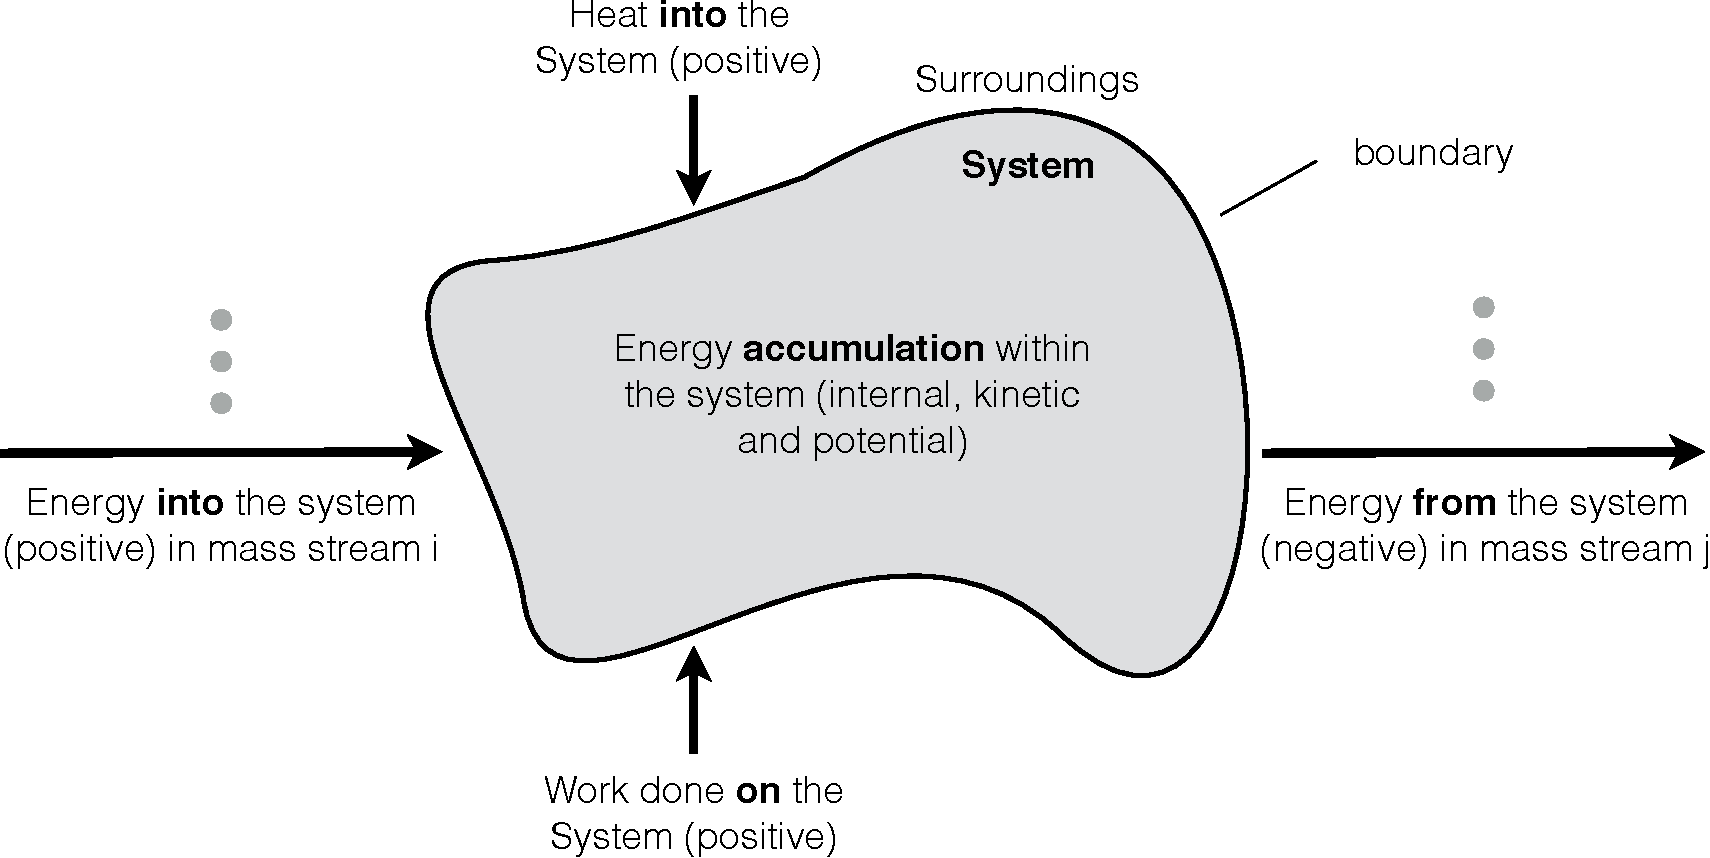
\includegraphics[width=0.80\textwidth]{./figs/EnergySchematic.pdf}
  \caption{Schematic of a general system and its surroundings. $\mathcal{S}$ streams enter or exit from the system which can transfer both heat and work with the surroundings.
  $\mathcal{R}$ chemical reactions can act a source or sink of heat for the system.}
  \label{fig-energy-schematic}
\end{figure}
Putting these ideas together we can write the \textit{differential} energy and mass balance equations of the form:
\begin{eqnarray}\label{eqn:energy-balance-precursor}
d\left(me\right)\Bigr|_{sys} &=& \delta{Q}+\delta{W}+\sum_{s=1}^{\mathcal{S}}\nu_{s}e_{s}\delta{m}_{s} + \sum_{r=1}^{\mathcal{R}}\delta E_{r}\\\label{eqn:material-balance-precursor}
dm &=& \sum_{s=1}^{\mathcal{S}}\nu_{s}\delta{m}_{s}
\end{eqnarray}where $e$ denotes the \textit{total} energy in the system per unit mass (or mol), $e_{s}$ denotes the \textit{total} energy of stream $s$ per unit mass (or mol),
$m$ and $m_{s}$ denote the system mass, and the mass of stream $s$ respectively, while $\delta E_{r}$ denotes the heat liberated or consumed by chemical reaction r.
Lastly, the quantity $\nu_{s}$ denotes a direction parameter for stream $s$; $\nu_{s}$ = 1 if stream $s$ enters the system, while $\nu_{s}$ = -1 if stream $s$ exits the system.

\paragraph*{What is $d\left(\cdot\right)$ versus $\delta\left(\cdot\right)$?}
A curious feature of Eqn \eqref{eqn:energy-balance-precursor} and \eqref{eqn:material-balance-precursor} is the $d\left(\cdot\right)$ versus the $\delta\left(\cdot\right)$ operators;
the $d\left(\cdot\right)$ operator denotes an \textit{exact} differential, while $\delta\left(\cdot\right)$ denotes an \textit{inexact} differential.
We'll talk more about this later, but an easy way to think about the difference between these operators is that exact differentials describe changes in system quantities,
while inexact differentials describes actions taken on the system (adding mass, adding heat etc).
Mathematically, integrals of exact differentials take the form:
\begin{equation}
\Delta x = \int_{x_{1}}^{x_{2}}dx
\end{equation}while integrals of inexact differentials are given by:
\begin{equation}
x = \int \delta x
\end{equation}

The differential energy and mass balance equations given by Eqn. \eqref{eqn:energy-balance-precursor} and \eqref{eqn:material-balance-precursor} can be converted to
the more familiar rate based balances by dividing both sides by a time window $\Delta{t}$ and allowing the window to shrink to zero ($\Delta{t}\rightarrow{0}$):
\begin{equation}
\frac{d}{dt}\left(me\right)\Bigr|_{sys} = \dot{Q}+\dot{W}+\sum_{s=1}^{\mathcal{S}}\nu_{s}e_{s}\dot{m}_{s}+ \sum_{r=1}^{\mathcal{R}}\dot{E}_{r}
\end{equation}where $\dot{Q},\dot{W},\dot{m}_{s}$ denote the rate of heat, work and mass input/output from the system in stream s.
Thus, the right-hand side describes the rate of accumulation of total energy in the system, while the left-hand side describes the various sources and sinks of total energy.
For most chemical engineering systems, we'll formulate total energy as the sum of the internal $U$, kinetic $E_{K}$ and potential energies $E_{P}$:
\begin{equation}
E = U + \frac{1}{2}ms_{j}^{2} + mgz
\end{equation} or on a per mass (mol) basis:
\begin{equation}
e = u + \frac{1}{2}s_{j}^{2} + gz
\end{equation}The total energy of any stream can also be represented as the sum of the internal, kinetic and potential energies of the molecules in that stream.
Putting these ideas together, we can write the general macroscopic energy and mass balances as:
\begin{eqnarray}\label{eqn:general-open-balance}
	\frac{d}{dt}\left[m\left(u+e_{K}+e_{P}\right)\right]\Bigr|_{sys} &=& \dot{Q}+\dot{W}+\sum_{s=1}^{\mathcal{S}}\nu_{s}\left(u_{s}+gz_{s}+\frac{1}{2}s_{s}^{2}\right)\dot{m}_{s}+\sum_{r=1}^{\mathcal{R}}\dot{E}_{r}\\\label{eqn:total-mass-balance}
	\frac{dm}{dt} = \sum_{s=1}^{\mathcal{S}}\nu_{s}\dot{m}_{s}
\end{eqnarray}

\section*{What is work in a thermodynamic system?}

\paragraph*{Work in a closed system.}
Let's begin by discussing expansion work in a \textit{closed} system (no exchange of material between the system and the surroundings).
In physics, a force does work if, when acting on a body, there is a displacement of the point of application in the direction of the force.
Work can be expressed by the relationship:
\begin{equation}\label{eqn:work-definition}
\delta{W} = \mathbf{F}\cdot d\mathbf{s}
\end{equation}where $\mathbf{F}$ denotes a force vector, and $d\mathbf{s}$ denotes a displacement vector. To calculate work using Eqn \eqref{eqn:work-definition},
we must take the scalar (dot or inner) product between the force vector and the displacement vector.
We can rewrite the force vector (and similarly the displacement vector) in terms of unit vectors $\mathbf{e}_{i}$ or:
\begin{equation}
\mathbf{F} = \sum_{i}F_{i}\mathbf{e}_{i}
\end{equation}where our unit vectors are \emph{orthonormal} to each other:
\begin{equation}
\mathbf{e}_{i}\cdot\mathbf{e}_{j} = \left(\mathbf{e}_{i},\mathbf{e}_{j}\right) = \left\{
\begin{array}{lr}
1 & : ~i=j \\
0 & : ~i\neq{j}
\end{array}
\right.
\end{equation}If we substitute the force and displacement vectors into Eqn \eqref{eqn:work-definition} (our definition of work) we arrive at:
\begin{equation}
\delta W = \sum_{i}\sum_{j} F_{i}ds_{j}\left(\mathbf{e}_{i},\mathbf{e}_{j}\right)
\end{equation}which simplifies to:
\begin{equation}\label{eqn:differential-work}
\delta W = \sum_{i} F_{i}ds_{i}
\end{equation}because we know that $\left(\mathbf{e}_{i},\mathbf{e}_{i}\right)$ = 1, and all other cases equal zero.

\begin{figure*}[!ht]\centering
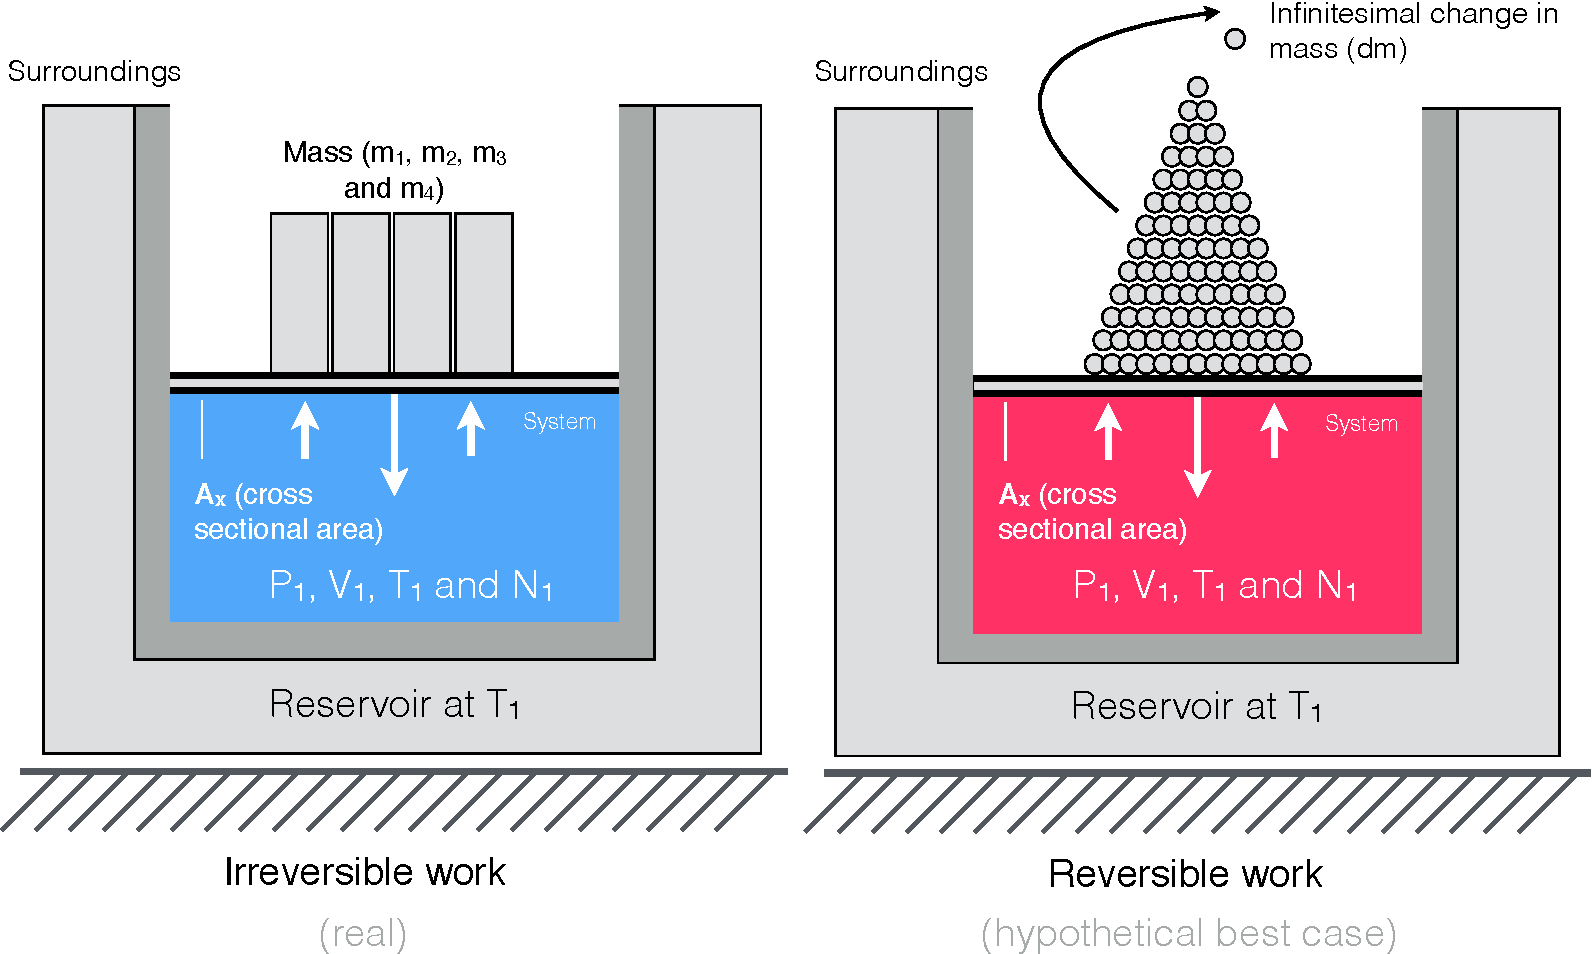
\includegraphics[width=0.60\textwidth]{./figs/WorkReversible.pdf}
\caption{Schematic of isothermal expansion work for a closed system for finite (irreversible) and hypothetically infinitesimal (reversible) changes in the external pressure.
}\label{fig-expansion-work-schematic}
\end{figure*}

We'll typically focus on \textit{reversible} pressure-volume expansion work shown schematically in Fig. \ref{fig-expansion-work-schematic}.
Imagine we have an isothermal chamber filled with an ideal gas at temperature T$_{1}$ that is being compressed by a weightless, frictionless piston loaded with total mass $M$.
At equilibrium, the gravitational external force pushing down on the piston $F_{e}$ will be counterbalanced by the force of the gas molecules hitting the piston, $F_{sys}$.
Force is related to pressure through an area, in this case the cross sectional area of the piston $A_{\perp}$, thus at equilibrium:
\begin{equation}
F_{sys}/A_{\perp} - F_{e}/A_{\perp} = 0
\end{equation}or $P_{sys} = P_{e}$.
Substituting the pressure into the differential work expression Eqn \eqref{eqn:differential-work} gives:
\begin{equation}\label{eqn:delta-w-almost}
\delta W = - P_{e}A_{\perp}ds_{2}
\end{equation}where we have no displacement in the x (s$_{1}$) or z (s$_{3}$) directions.
However, the product $A_{\perp}ds_{2}$ describes the displacement of an area, which is volume, thus Eqn. \eqref{eqn:delta-w-almost} becomes:
\begin{equation}
\delta W = - P_{e}dV
\end{equation}or after integration of the inexact differential:
\begin{equation}\label{eqn:work-equation}
W = - \int P_{e}dV
\end{equation}
Let's remove one of the weights, consider the case shown on the left of Fig. \ref{fig-expansion-work-schematic}.
Initially, the system is at rest and the pressures are equal.
However, when we remove a finite weight, there will be a mismatch between the system and surrounding pressure ($P_{sys}>P_{e}$)
causing the piston to accelerate upwards. Eventually the pressures will equilibrate, and the piston will come to rest.
This type of expansion work is called \textit{irreversible} (perhaps a better term would be non-static or non-equilibrium work).
When we were at equilibrium we knew $P_{sys}$, however, in between the equilibrium states for an irreversible expansion we do not know the system pressure.
Imagine instead that we do a hypothetical expansion in which we break the same weight $M$ into tiny particles of size $dM$, and remove a single particle at a time. This type of expansion is called \textit{reversible} (perhaps a better name would equilibrium or static work).
In this case, the equilibrium assumption remains approximately true, and at each hypothetical stage of the expansion $P_{sys}\simeq P_{e}$, thus:
\begin{equation}
W = - \int_{1}^{2} \frac{nRT}{V}dV
\end{equation}where we used the the ideal gas law $PV - nRT = 0$
to estimate the relationship the system pressure and volume. Evaluating the integral between state 1 (the start state) and some state 2 gives:
\begin{equation}\label{eqn:isothermal-reversible-expansion}
W = - nRT_{1}\ln\frac{V_{2}}{V_{1}}
\end{equation}
\begin{wrapfigure}{l}{0.50\textwidth}
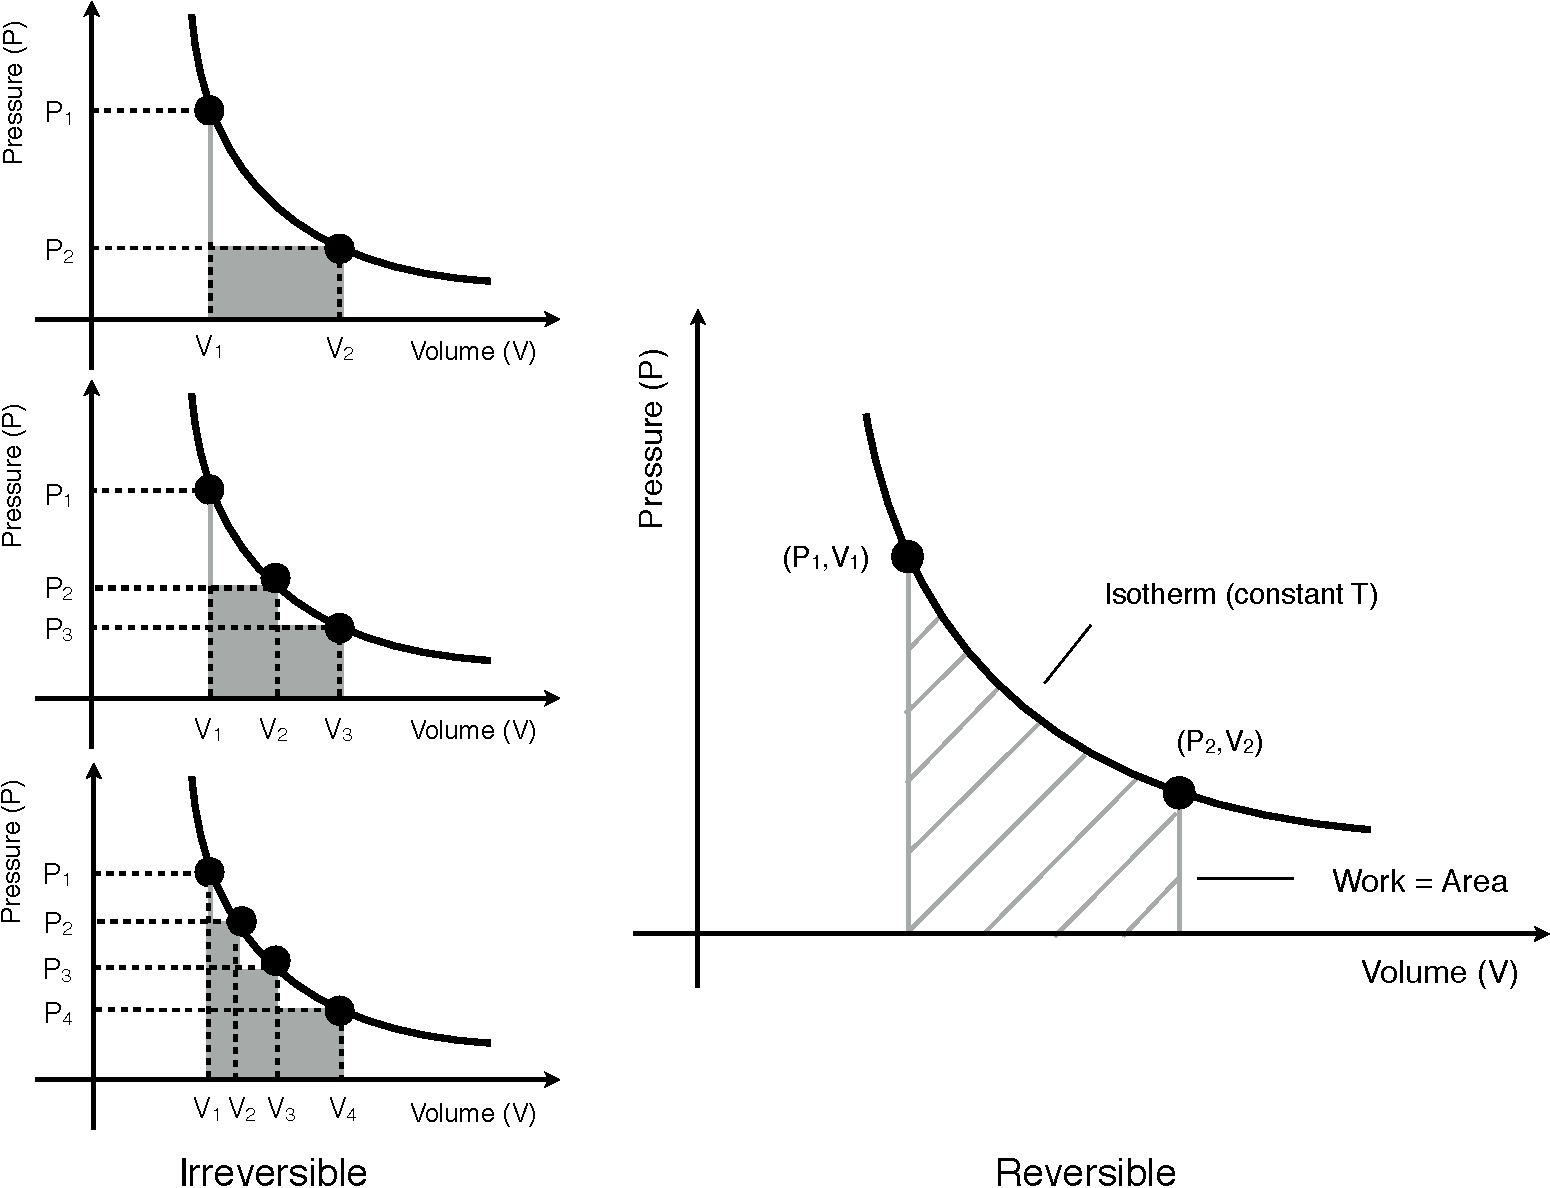
\includegraphics[width=0.49\textwidth]{./figs/WorkArea.pdf}
\caption{Schematic of the work generated by irreversible (left) and reversible (right) isothermal expansion of an ideal gas.
Reversible work generates the maximum possible work, but is a hypothetical upper bound.}\label{fig-expansion-work-area}
\end{wrapfigure}

Another way to think about expansion work is as an area under a curve.
From the definition Eqn \eqref{eqn:work-equation}, we see that work is also equal to the area under the curve in the P-V plane (Fig \ref{fig-expansion-work-area}).
Thus, finite changes in the opposing pressure (no longer in equilibrium with the surroundings) leads to jumps in the P-V plane (and missed work).
On the other hand, infinitesimally small changes in the surrounding pressure leads to a smooth expansion and the maximum possible work.
While reversible expansions are not real, we'll typically assume reversible behavior with the understanding that we are estimating the upper bound of system performance.

\paragraph*{Work in an open system.}
For an open system, we have \emph{shaft} and \emph{flow} work:
\begin{equation}
	\dot{W} = \dot{W}_{s} + \dot{W}_{f}
\end{equation}Shaft work $\dot{W}_{s}$ describes mechanically useful work, while flow work $\dot{W}_{f}$ is the energy required to push fluid into or from the system.
Thus, for an open system the total work is given by:
\begin{equation}\label{eqn:open-work}
	\dot{W} = \dot{W}_{s} + \sum_{s=1}^{\mathcal{S}}\nu_{s}\left(Pv\right)_{s}\dot{m}_{s}
\end{equation}where $P_{s}$ denotes the pressure of stream s, and $v_{s}$ denotes specific volume (e.g., L/kg or L/mol) of stream s.
Substituting Eqn. \eqref{eqn:open-work} into the energy balance Eqn. \eqref{eqn:general-open-balance} gives:
\begin{equation}
	\frac{d}{dt}\left[m\left(u+e_{K}+e_{P}\right)\right]\Bigr|_{sys} = \dot{Q}+\dot{W}_{s} + \sum_{s=1}^{\mathcal{S}}\nu_{s}\left\{\left(Pv\right)_{s}+e_{s}\right\}\dot{m}_{s}+ \sum_{r=1}^{\mathcal{R}}\dot{E}_{r}
\end{equation}If we collect terms and define a new thermodynamic quantity called the enthalpy $h$ ([J/mol] or [J/mass]) for stream j:
\begin{equation}
	h_{j} = u_{j} + \left(Pv\right)_{j}
\end{equation}we arrive at the total macroscopic energy balance for an open system:
\begin{eqnarray}
	\frac{d}{dt}\left[m\left(u+e_{K}+e_{P}\right)\right]\Bigr|_{sys} &=& \dot{Q}+\dot{W}_{s} + \sum_{s=1}^{\mathcal{S}}\nu_{s}\left(h+e_{K}+e_{P}\right)_{s}\dot{m}_{s} + \sum_{r=1}^{\mathcal{R}}\dot{E}_{r}\\
	\frac{dm}{dt} &=& \sum_{s=1}^{\mathcal{S}}\nu_{s}\dot{m}_{s}
\end{eqnarray}

\subsection*{Derivation of the first law of thermodynamics for a closed system.}
Let's begin by simplifying the differential energy and mass balances; consider a \textit{closed} system, with no chemical reactions consisting of a pure working fluid that obeys the general equation of state:
\begin{equation}
	\mathcal{F}\left(P,V,T,N\right) = 0
\end{equation}
In a closed system, $\delta{m}_{s}$ = 0 for all streams, and no chemical reactions says that $\sum_{r=1}^{\mathcal{R}}\delta E_{r}$ = 0. Thus, our energy and material balances reduce to:
\begin{eqnarray}\label{eqn:energy-balance-precursor-internal}
d\left(mu\right)\Bigr|_{sys} &=& \delta{Q}+\delta{W}\\\label{eqn:material-balance-precursor-internal}
dm &=& 0
\end{eqnarray}
Expanding the differential on the left hand side of the energy balance leads to:
\begin{equation}
md\left(u\right)\Bigr|_{sys}+ud\left(m\right)\Bigr|_{sys} = \delta{Q}+\delta{W}
\end{equation}We know that $dm$ = 0 (closed system), so the energy balance reduces to:
\begin{equation}\label{eqn:almost-first-law}
dU = \delta{Q}+\delta{W}
\end{equation}where we have dropped the explicit system reference and absorbed the mass. Eqn \eqref{eqn:almost-first-law} is the differential form of the \textit{first law of thermodynamics}.
We can derive the difference form by integrating both side of Eqn. \eqref{eqn:almost-first-law} from state 1 to 2 which gives:
\begin{equation}
\Delta{U} = Q + W
\end{equation}or on a specific basis:
\begin{equation}
\Delta{u} = q + w
\end{equation}
Solving for $\delta{Q}$ and substituting our definition of PV-work
\begin{equation}
\delta{W} = - PdV
\end{equation}
yields:
\begin{equation}\label{eqn:first-law-closed-system-differential}
	\delta{Q} = dU + PdV
\end{equation}where $P$ denotes the system pressure (assumed to be equilibrium with the surroundings) and V denotes the volume of the system.

\subsection*{Derivation of general heat capacity relationships.}
Imagine that we have a function that describes how the internal energy of a system varies with other thermodynamic states $x_{1},x_{2},\hdots,x_{N}$:
\begin{equation}
	U\left(x_{1},x_{2},\hdots,x_{N}\right) = 0
\end{equation}
We can take the \emph{total~differential} of of internal energy equation:
\begin{equation}
	dU = \sum_{j = 1}^{N}\left(\frac{\partial{U}}{\partial{x_{j}}}\right)_{x_{1},x_{2},\hdots,x_{N},j}dx_{j}
\end{equation}and substitute this into into Eqn. \eqref{eqn:first-law-closed-system-differential} to arrive at:
\begin{equation}\label{eqn:general-change-heat-balance}
	\delta{Q} = \sum_{j = 1}^{N}\left(\frac{\partial{U}}{\partial{x_{j}}}\right)\Bigr|_{x_{1},x_{2},\hdots,x_{N},j}dx_{j} + pdV
\end{equation}Eqn. \eqref{eqn:general-change-heat-balance} is a completely general equation that relates the change in heat ($\delta{Q}$) to
the equation of state for the internal energy of the system we are studying. For single component systems, the states $x_{1},x_{2},\hdots,x_{N}$ are combinations of
four variables, temperature, pressure, volume and abundance (the number of particles in the system). Since we have a closed system, and we have no chemical reactions
our list of state variable is simply the temperature, pressure and volume. If we specify two of these variables we can calculate the third from the state equation.
This leads to three possible system configurations (for a constant abundance system):
\begin{itemize}
	\item{$\left(T,V\right)$ systems: If the independent state variables are temperature $T$ and volume $V$, we can the write $dU$ as:
	\begin{equation}
		dU = \left(\frac{\partial{U}}{\partial{T}}\right)_{V}dT + \left(\frac{\partial{U}}{\partial{V}}\right)_{T}dV
	\end{equation}which yields a differential energy balance of the form:
	\begin{equation}\label{eqn:T-V-N-system}
		\delta{Q} = \left(\frac{\partial{U}}{\partial{T}}\right)_{V}dT + \left[\left(\frac{\partial{U}}{\partial{V}}\right)_{T} + p\right]dV
	\end{equation}}

	\item{$\left(T,P\right)$ systems: If the independent state variables are pressure $P$ and temperature $T$, we can write $dU$ as:
	\begin{equation}
		dU = \left(\frac{\partial{U}}{\partial{T}}\right)_{P}dT + \left(\frac{\partial{U}}{\partial{P}}\right)_{T}dP
	\end{equation}which yields a differential energy balance of the form:
	\begin{equation}\label{eqn:T-P-N-system}
		\delta{Q} = \left[\left(\frac{\partial{U}}{\partial{T}}\right)_{P}+P\left(\frac{\partial{V}}{\partial{T}}\right)_{P}\right]dT +
		\left[\left(\frac{\partial{U}}{\partial{P}}\right)_{T} + p\left(\frac{\partial{V}}{\partial{P}}\right)_{T}\right]dP
	\end{equation}where we have assumed:
	\begin{equation}
		dV = \left(\frac{\partial{V}}{\partial{T}}\right)_{P}dT+\left(\frac{\partial{V}}{\partial{P}}\right)_{T}dP
	\end{equation}}

	\item{$\left(P,V\right)$ systems: If the independent state variables are pressure $P$ and volume $V$, we can write $dU$ as:
	\begin{equation}
		dU = \left(\frac{\partial{U}}{\partial{P}}\right)_{V}dP + \left(\frac{\partial{U}}{\partial{V}}\right)_{P}dV
	\end{equation}which yields a differential energy balance of the form:
	\begin{equation}
		\delta{Q} = \left(\frac{\partial{U}}{\partial{P}}\right)_{V}dP + \left[\left(\frac{\partial{U}}{\partial{V}}\right)_{P} + p\right]dV
	\end{equation}}

\end{itemize}

\begin{wrapfigure}{r}{0.60\textwidth}
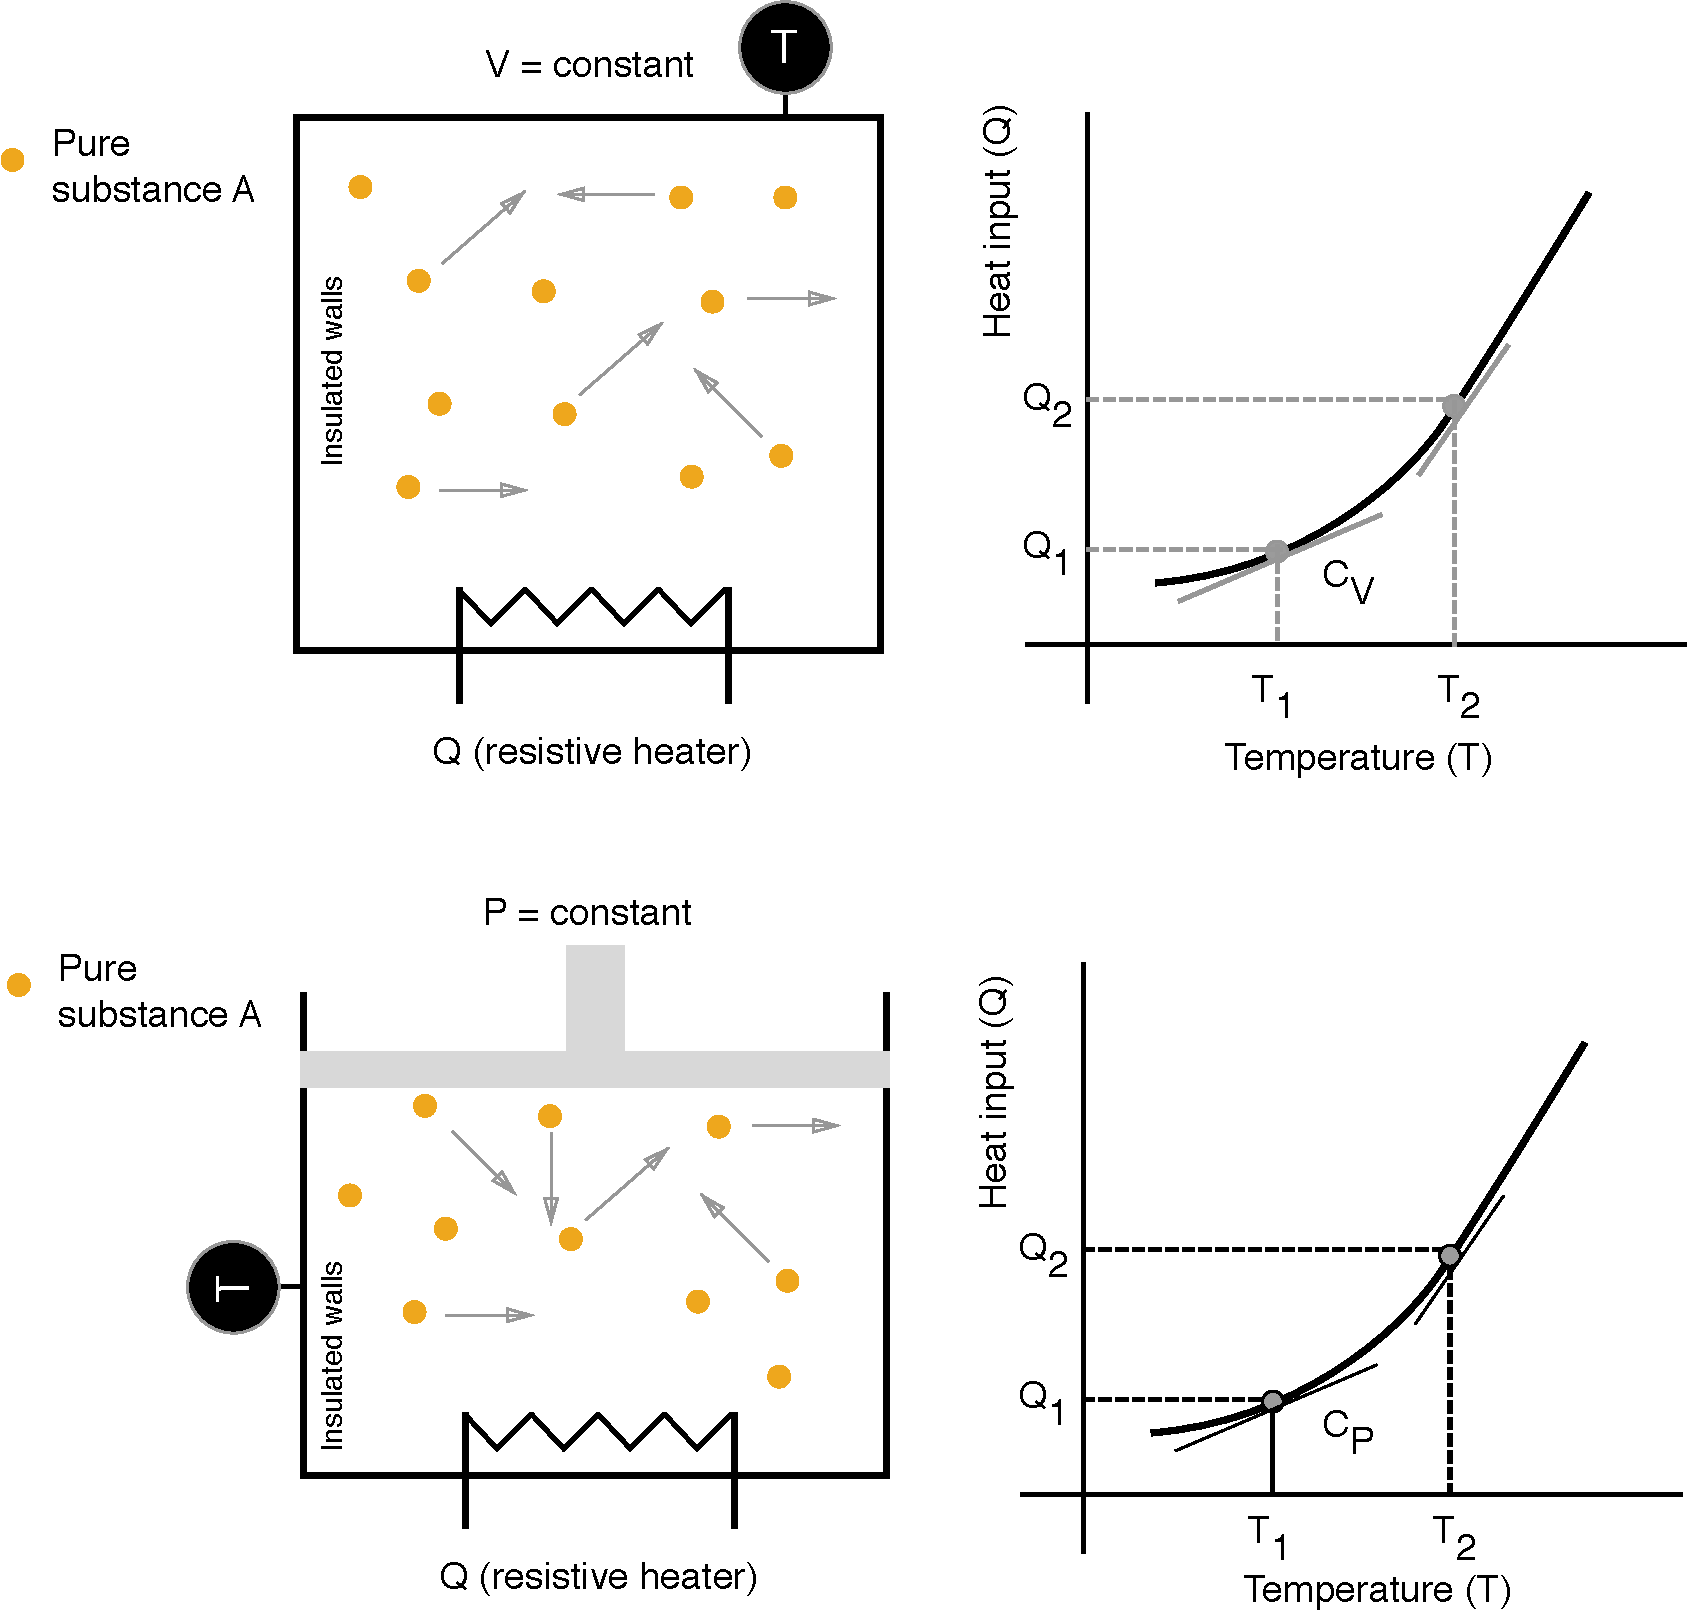
\includegraphics[width=0.55\textwidth]{./figs/HeatCapacity-eps-converted-to.pdf}
\caption{Schematic of the experimental setup for a constant volume (top) and a constant pressure (bottom) heat capacity experiment for a pure substance A.}\label{fig-heat-capacity}
\end{wrapfigure}


\subsection*{Changes in internal energy at constant volume. Definition of $C_{V}$.}
Let's assume that we are using a $\left(T,V\right)$ system with a pure substance. When we supply heat at a constant volume (Fig. \ref{fig-heat-capacity}, top),
Eqn \eqref{eqn:T-V-N-system} reduces to:
\begin{equation}
	\delta{Q} = \left(\frac{\partial{U}}{\partial{T}}\right)_{V}dT
\end{equation}where $dV = 0$. If we divide both sides by $dT$, we arrive at an expression which describes how the internal energy changes with temperature:
\begin{equation}\label{eqn:constant-volume-heat-capacity}
	C_{V} \equiv \frac{\delta{Q}}{dT} = \left(\frac{\partial{U}}{\partial{T}}\right)_{V}
\end{equation}where the subscript $V$ denotes the derivatives are calculated at constant volume. The quantity $C_{V}$ is called the constant volume heat capacity.
The term $\delta{Q}/{dT}$ (and hence the heat capacity) can easily be measured experimentally (Fig \ref{fig-heat-capacity}). If we integrate both sides of
Eqn. \eqref{eqn:constant-volume-heat-capacity} with respect to temperature, we arrive at:
\begin{equation}
	\Delta{U} = \int_{T_{1}}^{T_{2}}C_{V}dT
\end{equation}Note that $C_{V}$ is typically a strong function of temperature, so if $T_{1}$ and $T_{2}$ span a large temperature range, we \textit{cannot} pull $C_{V}$ out the integral.
Instead, we have to estimate how $C_{V}$ varies with temperature, for example estimating $C_{V}$ at many different temperatures and then fitting the results to function of temperature.

\subsection*{Changes in internal energy at constant pressure. Definition of $C_{P}$.}
For a constant pressure system, let's start with Eqn. \eqref{eqn:T-P-N-system}. When we supply heat at a constant pressure (Fig. \ref{fig-heat-capacity}, bottom) $dP = 0$,
which reduces Eqn. \eqref{eqn:T-P-N-system} to:
\begin{equation}
	\delta{Q}_{P} = \left[\left(\frac{\partial{U}}{\partial{T}}\right)_{P}+P\left(\frac{\partial{V}}{\partial{T}}\right)_{P}\right]dT
\end{equation}If we divide both sides of the constant pressure $\delta{Q}_{P}$ expression by $dT$ we arrive at:
\begin{equation}\label{eqn:almost-cp}
	\frac{\delta{Q}_{P}}{dT} = \left(\frac{\partial{U}}{\partial{T}}\right)_{P}+P\left(\frac{\partial{V}}{\partial{T}}\right)_{P}
\end{equation}The right-hand side of Eqn. \eqref{eqn:almost-cp} is the sum of an internal energy term and a constant pressure expansion term, which is similar to our definition of
enthalpy:
\begin{equation}\label{eqn:enthalpy}
	H \equiv U + PV
\end{equation}Computing the total differential of $H$ yields:
\begin{equation}
	dH = dU + PdV + VdP
\end{equation}However, we are at constant pressure ($dP = 0$), which reduces the enthalpy differential to:
\begin{equation}\label{eqn:enthalpy-differential-constant-pressure}
	dH = dU + PdV
\end{equation}Differentiating both sides of Eqn. \eqref{eqn:enthalpy-differential-constant-pressure} with respect to temperature (at constant pressure) gives the expression:
\begin{equation}
	\left(\frac{\partial{H}}{\partial{T}}\right)_{P} = \left(\frac{\partial{U}}{\partial{T}}\right)_{P} + P\left(\frac{\partial{V}}{\partial{T}}\right)_{P}
\end{equation}Thus, the change in the internal energy of a material as a function of temperature, when measured at constant pressure, is equal to the change in enthalpy:
\begin{equation}\label{eqn:constant-pressure-heat-capacity}
	C_{P}\equiv\frac{\delta{Q}_{P}}{dT} = \left(\frac{\partial{H}}{\partial{T}}\right)_{P}
\end{equation}Similar to the constant volume heat capacity, we can decompose Eqn. \eqref{eqn:constant-pressure-heat-capacity} to solve for the change in enthalpy resulting
from a change in temperature (at a constant pressure):
\begin{equation}
	\Delta{H} = \int_{T_{1}}^{T_{2}}C_{P}dT
\end{equation}Also like the constant volume heat capacity, $C_{P}$ can be a strong function of $T$, thus, we typically cannot pull it out the temperature integral for large changes
in temperature.

\subsection*{Is there a relationship between $C_{V}$ and $C_{P}$?}
Intuitively, given the same pure substance and the same heat input, you would expect that there is a relationship between $C_{V}$ and $C_{P}$. To explore this question, let's consider
the first-law written for a $(T,V)$ system held at a constant pressure $P$:
\begin{equation}\label{eqn:first-law-T-V-constant-P}
	\delta{Q}_{P} = \left(\frac{\partial{U}}{\partial{T}}\right)_{V}dT + \left[\left(\frac{\partial{U}}{\partial{V}}\right)_{T} + P\right]dV
\end{equation}Using our definition of the constant volume heat capacity, we can rewrite Eqn. \eqref{eqn:first-law-T-V-constant-P} as:
\begin{equation}
	\delta{Q}_{P} = C_{V}dT + \left[\left(\frac{\partial{U}}{\partial{V}}\right)_{T} + P\right]dV
\end{equation}which, after differentiating with respect to temperature at a constant pressure becomes:
\begin{equation}\label{eqn:first-law-T-V-constant-P-almost-there}
	\frac{\delta{Q}_{P}}{dT} = C_{V} + \left[\left(\frac{\partial{U}}{\partial{V}}\right)_{T} + P\right]\frac{\partial{V}}{\partial{T}}_{P}
\end{equation}Again, using our definition of constant pressure heat capacity this time, Eqn. \eqref{eqn:first-law-T-V-constant-P-almost-there} reduces to:
\begin{equation}\label{eqn:heat-capacity-relationship}
	C_{P} - C_{V} = \left[\left(\frac{\partial{U}}{\partial{V}}\right)_{T} + P\right]\left(\frac{\partial{V}}{\partial{T}}\right)_{P}
\end{equation}

Equation \eqref{eqn:heat-capacity-relationship} governs the general relationship between $C_{P}$ and $C_{P}$ for an arbitrary pure material.
Although we have not (yet) explicitly shown it, the quantity of the right-hand side of Eqn. \eqref{eqn:heat-capacity-relationship} is always greater than zero, thus $C_{P}>{C_{V}}$.
To work out the exact difference between the heat capacities, we need an equation of state for the material we are exploring.
Right now, we only have this relationship for an ideal gas. We know that the internal energy of an ideal gas is given by:
\begin{equation}
	U = \frac{3}{2}Nk_{B}T
\end{equation}Thus, the first term on the right side of Eqn. \eqref{eqn:heat-capacity-relationship} vanishes i.e., $\left(\partial{U}/\partial{V}\right)_{T} = 0$ because
$U$ is only a function of $T$. This leaves us with the volume expansion term:
\begin{equation}\label{eqn:CP-CV-relationship-ideal-gas-almost}
	C_{P} - C_{V} = P\left(\frac{\partial{V}}{\partial{T}}\right)_{P}
\end{equation}Rearranging the ideal gas law for $V$, and differentiating with respect to temperature $T$ yields:
\begin{equation}
	\left(\frac{\partial{V}}{\partial{T}}\right)_{P} = \frac{nR}{P}
\end{equation}which, when substituted into Eqn. \eqref{eqn:CP-CV-relationship-ideal-gas-almost}, yields:
\begin{equation}
	C_{P} - C_{V} = nR
\end{equation}where $n$ denotes the number of mols of ideal gas, and $R$ denotes the ideal gas constant.

\begin{wrapfigure}{l}{0.59\textwidth}
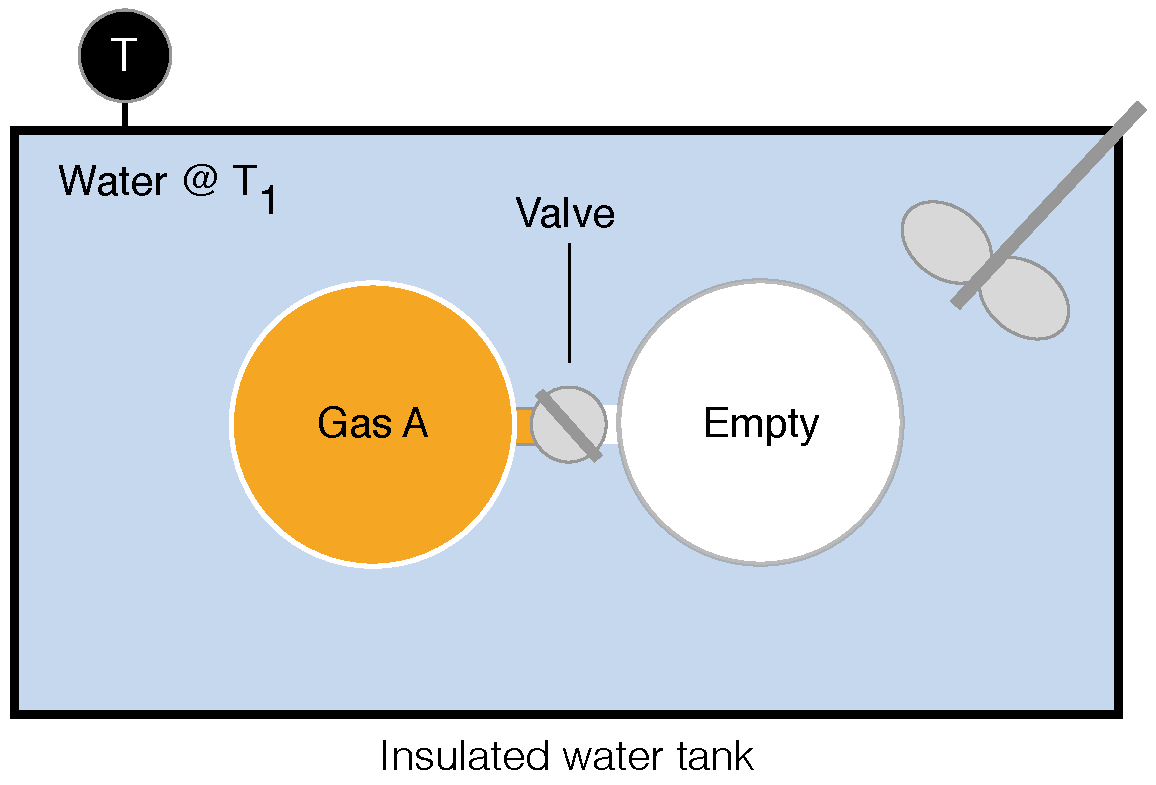
\includegraphics[width=0.58\textwidth]{./figs/JouleExpansion.pdf}
\caption{Schematic of the experimental apparatus used in a Joule free expansion experiment.
Two identical containers, separated by a valve, are in thermodynamic equilibrium with an insulated water bath initially at temperature $T_{1}$.
Container A is filled with a gas, while container B is initially empty.
At time = 0, the valve is opened an the gas from container A expands into container B.}\label{fig-joule-expansion}
\end{wrapfigure}

\subsection*{Does the internal energy of a material change with the volume of the container?}
Theoretically, the internal energy of a material may also be a function of the volume of the system. This is governed by the partial derivative $\left(\partial{U}/\partial{V}\right)_{T}$ in
our internal energy expansion. However, unlike heat capacity, $\left(\partial{U}/\partial{V}\right)_{T}$ is not as easy to measure experimentally.
The classic experimental technique to measure this quantity is called a \textit{Joule~free~expansion} (Fig. \ref{fig-joule-expansion}).
In this experiment, two identical containers, separated by a valve, are immersed in a constant temperature water bath.
Container A is filled with a gas, while container B is initially empty. At time = 0, the valve is opened an the gas from container A expands into container B.
Joule measured the temperature of the water bath \textit{before} he opened the valve, and again after the system was allowed to come to thermal equilibrium.
There was \textit{no} change in the temperature of the water bath. Let's try and interpret this result using our understanding of energy transfer and the macroscopic total
energy balance. Starting from the macroscopic energy balance for a closed system in differential form, we have:
\begin{equation}
	dU = \delta{Q} + \delta{W}
\end{equation}While the gas expands from container A into container B, $\delta{W} = 0$ as the gas particles are expanding against zero opposing pressure.
Additionally, since the temperature of the \textit{finite} water bath was unchanged it follows that $\delta{Q} = 0$, thus $dU = 0$.
We also know that:
\begin{equation}
	dU = \left(\frac{\partial{U}}{\partial{T}}\right)_{V}dT + \left(\frac{\partial{U}}{\partial{V}}\right)_{T}dV = 0
\end{equation}However, $dT = 0$ which implies:
\begin{equation}
	dU = \left(\frac{\partial{U}}{\partial{V}}\right)_{T}dV = 0
\end{equation}Since $dV\neq{0}$ (the volume of our system approximately doubled), this means:
\begin{equation}\label{eqn:joule-expansion-result}
	\left(\frac{\partial{U}}{\partial{V}}\right)_{T} = 0
\end{equation}Equation \eqref{eqn:joule-expansion-result} says that the internal energy of a material is \textit{not} a function of volume. This finding is exactly true for an
ideal gas (since we derived the functional form for the internal energy), however, it is not true for a real gas (it usually a small positive value for real gases).

\end{document}
